\documentclass{beamer}
%
% Choose how your presentation looks.
%
% For more themes, color themes and font themes, see:
% http://deic.uab.es/~iblanes/beamer_gallery/index_by_theme.html
%
\mode<presentation>
{
  \usetheme{Boadilla}      % or try Darmstadt, Madrid, Warsaw, ...
  \usecolortheme{beaver} % or try albatross, beaver, crane, ...
  \usefonttheme{default}  % or try serif, structurebold, ...
  \setbeamertemplate{navigation symbols}{}
  \setbeamertemplate{caption}[numbered]
  
} 

\usepackage{xcolor,colortbl}
\usepackage[english]{babel}
\usepackage[utf8x]{inputenc}
\usepackage{courier}
\usepackage{dsfont}
\usepackage{verbatim} 
\usepackage{enumerate}
\usepackage{tikz}
\usepackage{multirow}
\usepackage{bbm}
\usepackage{amsmath}
\usepackage{venndiagram}
\usepackage{epigraph} 
%\usepackage{xcolor}

%\usepackage{enumitem}

\usepackage{hyperref}
\hypersetup{
    colorlinks=true,
    linkcolor=blue,
    filecolor=magenta,      
    urlcolor=cyan,
}

% R stuff!
\usepackage{listings}
\definecolor{codegreen}{rgb}{0,0.6,0}
\definecolor{codegray}{rgb}{0.5,0.5,0.5}
\definecolor{codepurple}{rgb}{0.58,0,0.82}
\definecolor{backcolour}{rgb}{0.95,0.95,0.92}

\lstdefinestyle{mystyle}{
    backgroundcolor=\color{backcolour},    
    commentstyle=\color{codegreen},
    keywordstyle=\color{black},
    numberstyle=\tiny\color{codegray},
    stringstyle=\color{codepurple},
    basicstyle=\ttfamily\footnotesize,
    breakatwhitespace=false,         
    breaklines=true,                 
    captionpos=b,                    
    keepspaces=true,                 
    numbers=left,                    
    numbersep=5pt,                  
    showspaces=false,                
    showstringspaces=false,
    showtabs=false,                  
    tabsize=2
}

\lstset{style=mystyle}



%% Size options for nested itemized lists
\usepackage{relsize}
\setbeamerfont{itemize/enumerate body}{parent=normal text}
\setbeamerfont{itemize/enumerate subbody}{parent=normal text,size=\relsize{-1}}
%\setbeamerfont{itemize/enumerate subsubbody}{parent=normal text,size=\relsize{-1}}




\setbeamertemplate{enumerate items}[default]
\setbeamertemplate{itemize item}[triangle]

%\setitemize{label=\usebeamerfont*{itemize item}%
%  \usebeamercolor[fg]{itemize item}
%  \usebeamertemplate{itemize item}}


\usetikzlibrary{shapes,decorations,arrows,calc,arrows.meta,fit,positioning}
\tikzset{
    -Latex,auto,node distance =1 cm and 1 cm,semithick,
    state/.style ={ellipse, draw, minimum width = 0.7 cm},
    point/.style = {circle, draw, inner sep=0.04cm,fill,node contents={}},
    bidirected/.style={Latex-Latex,dashed},
    el/.style = {inner sep=2pt, align=left, sloped}
}

\newcommand{\Mypm}{\mathbin{\tikz [x=1.4ex,y=1.4ex,line width=.1ex] \draw (0.0,0) -- (1.0,0) (0.5,0.08) -- (0.5,0.92) (0.0,0.5) -- (1.0,0.5);}}%



%% For block quote
\usepackage{etoolbox}
\AtBeginEnvironment{quote}{\par\singlespacing\small}


\title[Introduction to Statistics)]{$\chi^2$ Tests of Independence}
\subtitle{}
%\author{}
\author{Grinnell College}
\date{November 26, 2024}

\graphicspath{{img/}}

\begin{document}

\begin{frame}
  \titlepage
\end{frame}

\begin{frame}{Warm-up}
\begin{enumerate}
\item Suppose I flip a fair coin twice:
\begin{itemize}
\item What is the probability that I flip 0 heads?
\item Probability of one heads?
\item Probability of two heads?
\end{itemize} \vspace{8mm}
\item Suppose I repeat this twice flipping experiment 100 times. Of these I get 28, 55, and 17 instances of 0, 1, and 2 heads, respectively:
\begin{itemize}
\item Create a table of observed and expected values under the null hypothesis that my coin is fair
\item Using your table, construct a $\chi^2$ test statistic
\item From p-value, what conclusion would you make regarding our null hypothesis?
\end{itemize}
\end{enumerate}
\end{frame}

\begin{frame}
\begin{table}[ht]
\centering
\begin{tabular}{rrrrr}
  \hline
 & 0H & 1H & 2H & Total\\
  \hline
Expected & 25 & 50 & 25 & 100 \\ 
  Observed & 28 & 55 & 17 & 100 \\ 
   \hline
\end{tabular}
\end{table} \vspace{4mm}

\begin{align*}
\chi^2 &= \sum_{i=1}^k \frac{(\text{Expected}_i - \text{Observed}_i)^2}{\text{Expected}_i} \\[1em]
&= \frac{(25-28)^2}{25} + \frac{(50-55)^2}{50} + \frac{(25-17)^2}{25}\\[1em]
&= 3.42
\end{align*}
\end{frame}


\begin{frame}
\begin{center}
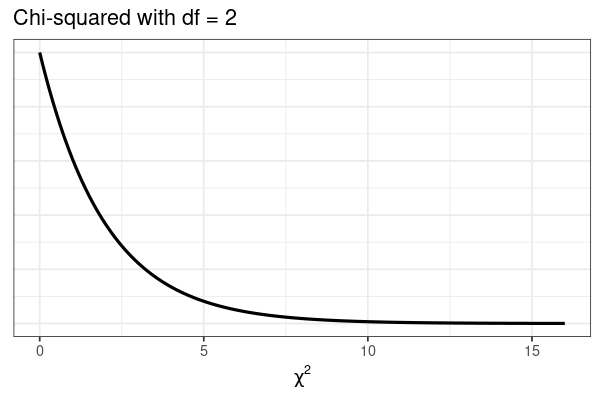
\includegraphics[scale=0.5]{chi1.png}
\end{center}
\end{frame}

\begin{frame}
\begin{center}
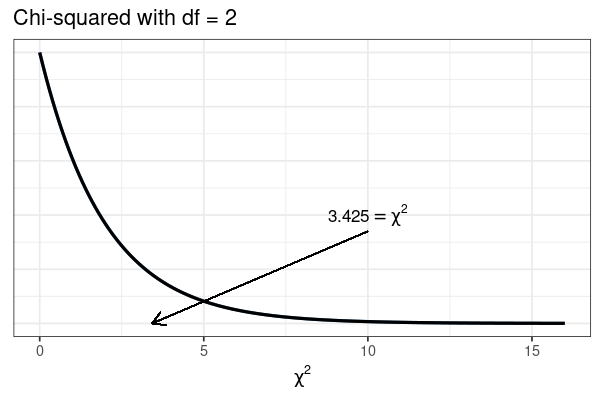
\includegraphics[scale=0.5]{chi2.png}
\end{center}
\end{frame}


\begin{frame}
\begin{center}
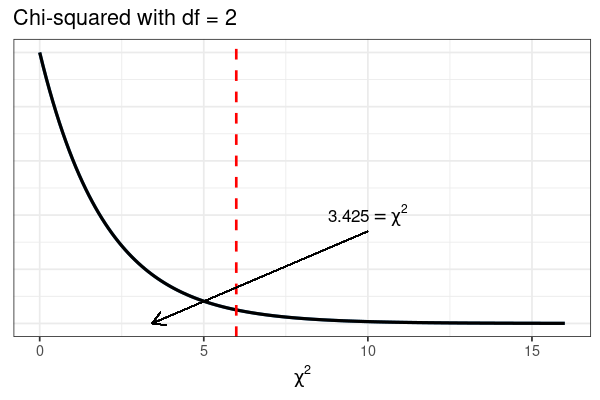
\includegraphics[scale=0.5]{chi3.png}
\end{center}
\end{frame}

\begin{frame}
\begin{center}
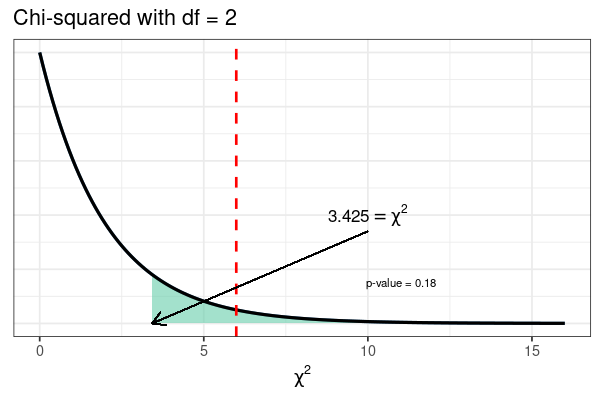
\includegraphics[scale=0.5]{chi4.png}
\end{center}
\end{frame}

\begin{frame}{$\chi^2$ Goodness of Fit}

Last class we introduced the $\chi^2$ \textbf{Goodness of Fit} test for assessing the goodness of fit for a single categorical variable
\begin{itemize}
    \item compares Observed data to Expected data (under $H_0$)
    \item $H_A$: proportions are not equal to specified values
\end{itemize}
\vspace{8mm}

We extend this today to the $\chi^2$ \textbf{Test of Independence} used to test the independence or lack of association between two categorical variables 
\begin{itemize}
    \item $H_0$ there is \textit{not} an association
    \item $H_A$: there is an association
\end{itemize}\vspace{6mm}

Calculating the test statistic for both of these is the same, we just need to keep track of the different Hypotheses and different df

\end{frame}

\begin{frame}{Independence and Probability}
Recall that, in general, the probability of two events $A$ and $B$ is given as
\begin{align*}
P(A \text{ and } B) = P(A|B)P(B) = P(B|A)P(A)
\end{align*}
with indepenedence \textit{if and only if (iff)}
\begin{align*}
P(A \text{ and } B) = P(A)P(B)
\end{align*} \vspace{4mm}

Next part: How does this translate to  a null hypothesis of independence between groups
\end{frame}

\begin{frame}
Suppose we have Cars and Trucks that can be painted either Blue or Red. We could represent these variables as such:
\begin{table}[ht]
\centering
\begin{tabular}{rcc|c}
  \hline
 & Red & Blue & Total\\
  \hline
Car & $n_1$ & $n_2$ &  $n_1+n_2$ \\ 
Truck & $n_3$ &  $n_4$ & $n_3+n_4$ \\ 
   \hline
Total & $n_1 + n_3$ & $n_2 + n_4$ & $N$ \\ \hline
\end{tabular}
\end{table}
The table above gives us the following information (for example):
\begin{itemize}
\item There are $n_1 + n_2$ vehicles that are cars
\item There are $n_2+n_4$ blue vehicles
\item There are $n_3$ blue trucks
\end{itemize}
We can use this to establish our null hypothesis
\end{frame}


\begin{frame}
\begin{table}[ht]
\centering
\begin{tabular}{rcc|c}
  \hline
 & Red & Blue & Total\\
  \hline
Car & $n_1$ & $n_2$ &  $n_1+n_2$ \\ 
Truck & $n_3$ &  $n_4$ & $n_3+n_4$ \\ 
   \hline
Total & $n_1 + n_3$ & $n_2 + n_4$ & $N$ \\ \hline
\end{tabular}
\end{table}
If our variables were independent, then our \textit{expected probability} is
\begin{align*}
P(\text{Car and Red}) &= P(\text{Car})P(\text{Red}) \\
&= \left(\frac{n_1 + n_2}{N} \right) \times \left(\frac{n_1 + n_3}{N} \right) 
\end{align*}
To get our expected counts, we would multiply this probability by $N$, the total number of observations:
\begin{align*}
\text{Expected Number of Red Cars} &= N \times  \left(\frac{n_1 + n_2}{N} \right) \times \left(\frac{n_1 + n_3}{N} \right) \\
&= \frac{(n_1 + n_3)(n_1 + n_2)}{N} 
\end{align*}
In other words, our \textit{expected counts} is the product of the row and column margins, divided by the total number of observations
\end{frame}

\begin{frame}{Expected Counts}
For example, suppose we had 60 cars, 40 trucks, 50 blue vehicles, and 50 red vehicles. The margins totals would look like this:
\begin{table}[ht]
\centering
\begin{tabular}{rcc|c}
  \hline
 & Red & Blue & Total\\
  \hline
Car &  &  & 60 \\ 
Truck &  &  & 40\\ 
   \hline
Total & 50 & 50 & 100 \\ \hline
\end{tabular}
\end{table}
From this, we have the following probabilities:
\begin{align*}
P(\text{Red}) = \frac{50}{100} = 0.5, \quad P(\text{Car}) = \frac{60}{100} = 0.6
\end{align*}
Under the null hypothesis of independence, the probability of both is
\begin{align*}
P(\text{Car and Red}) &= P(\text{Car})P(\text{Red}) = 0.5 \times 0.6 = 0.3
\end{align*}
Since there are 100 vehicles, and the probability of of a vehicle being a red car is 0.3, the expected number of red cars would be 30
\end{frame}

\begin{frame}{Expected Counts}
We could take our expected counts:
\begin{table}[ht]
\centering
\begin{tabular}{rcc|c}
  \hline
 & Red & Blue & Total\\
  \hline
Car & 30 & 30 & 60 \\ 
Truck & 20 & 20 & 40\\ 
   \hline
Total & 50 & 50 & 100 \\ \hline
\end{tabular}
\end{table}
And compare them to what we observe:
\begin{table}[ht]
\centering
\begin{tabular}{rcc|c}
  \hline
 & Red & Blue & Total\\
  \hline
Car & 32 & 28 & 60 \\ 
Truck & 18 & 22 & 40\\ 
   \hline
Total & 50 & 50 & 100 \\ \hline
\end{tabular}
\end{table}
\begin{align*}
\chi^2 &=  \frac{(30-32)^2}{30} + \frac{(30-28)^2}{30}+\frac{(20-18)^2}{20} + \frac{(20-22)^2}{20} = 0.735
\end{align*}
\end{frame}


\begin{frame}{Degrees of Freedom}
Just as with the univariate case, the $\chi^2$ test of independence is governed by its degrees of freedom \\ \vspace{4mm}

For a table with $k$ columns and $m$ rows, the total degrees of freedom is  $df = (k-1)\times(m-1)$ \\ \vspace{8mm}

The degrees of freedom for the car example, then would be $(2-1) \times(2-1) = 1$ \\ \vspace{8mm}

The process of finding critical values or $p$-values then proceeds identically as before 

\end{frame}

\begin{frame}{Review}

Here are the things to know about the test for independence:
\begin{itemize}
\item Expected counts come from products of margin probabilities
\item Degrees of freedom for $k$ columns and $m$ rows is $(k-1) \times (m-1)$
\item Everything else works the exact same way as the Goodness of Fit test
\item The main difference is that the \textit{null hypothesis} comes directly from the assumption of independence
\end{itemize}
\end{frame}

%
%\begin{frame}
%
%Until now, we have primarily used the Central Limit Theorem for hypothesis testing related to categorical data: \\
%
%\begin{itemize}
%\item One sample $Z$ test of the form $H_0: p = p_0$
%\item Two sample difference in proportion tests, i.e., $H_0: p_1 - p_2 = 0$
%\end{itemize}
%%\vspace{6mm}
%%In both of these tests, our outcome of interest was \textit{binary}, with probabilities or proportions given in terms of success or failure
%\end{frame}
%
%\begin{frame}{Categorical Data}
%Recall that categorical variables come in two different type: \textit{nominal} and \textit{ordinal} data \vpsace{3mm}
%
%Nominal data is such that the categories involved have no natural ordering, i.e., geographic region, sex, vehicle class, etc., 
%
%
%\end{frame}
%
%\begin{frame}
%Recall categorical variable, 2 types, nominal and ordinal. we doing nominal \\
%
%And actually, kinda like binomial. If I know prob of heads is 0.5, then automatically tails is 0.5 \\
%
%What if we are looking at [blood type]. knowing that 45\% is O tells us nothing about the rest. Or rather, I want to ask questions about proportions generally
%\end{frame}
%
%\begin{frame}
%start with one cateogrical variable case. Consider exam with 400 questions and ABCDE possible answers. we might want to check that P(A) = P(B) = ...
%
%That is, if it was exactly true we would have this table
%
%
%\end{frame}
%
%\begin{frame}
%As we have seen, there is variation in sample. That is, we could generate answers with same probability and still end up with some variation. For example this or this or this. That is, if our ``null" hypo is true, these are all well within realms of possibility. What we need then is test statistic (like t-test) and a reference distribution (like t or normal)
%\end{frame}
%
%\begin{frame}
%Introduce chi sq statistic it looks like this \\
%
%For reasons we will not worry about \\
%
%But a fun thing to note, this is actually just a squared sum normal distribution
%\end{frame}
%
%\begin{frame}
%Here, look at this distribution! Also for now note df = 1 (we will return to this in a bit) \\
%
%But we can compute our chi sq statistic and compare with null distribution to determine if this was likely or not
%\end{frame}
%
%\begin{frame}
%Ok resolve our ACT problem or whatever
%\end{frame}
%
%\begin{frame}
%To be clear, we don't have to assume that they are all equal, our null hypo can have the percentages of each group be whatever, and we can check against that \\
%
%For example, consider racial breakup of blah blah county. If we selected jurors randomly, the percentages of each race in juror pool should match what we see here. \\
%
%So here is $N$ (a total) and an expected percentage, we multiple to get expected values. \\
%
%Then here is what we observed, lets calculate this BITCH
%\end{frame}
%
%\begin{frame}
%Tests with a single variable called goodness of fit tests, i.e., how well does this data fit to what we should expect \\
%
%HOW IS THIS SIMILAR TO DIFFERENCE IN PROPS \\
%
%The distribution for this, regardless of how many groups will be $\chi^2$ with df = c-1
%\end{frame}

%%%%%%%%%%%%%%%%

%\begin{frame}
%\begin{columns}
%
%  \begin{column}{0.45\textwidth}
%%
%  \end{column}
%  \begin{column}{0.45\textwidth}
%%
%  \end{column}
%
%\end{columns}
%\end{frame}


\end{document}
